%\svnkwsave{$RepoFile: siminos/blog/energy.tex $}
%\svnidlong {$HeadURL$}
%{$LastChangedDate$}
%{$LastChangedRevision$} {$LastChangedBy$}
%\svnid{$Id$}

\chapter{Energy, dissipation, invariant moments}
\label{c-energy}

\renewcommand{\ssp}{x}             % state space point

\begin{description}
\item[2008-06-26 PC] moved this to Siminos thesis from
        \texttt{blog/flotsam.tex}.
\item[2009-10-02 PC] moved this back again from
        \texttt{blog/flotsam.tex}.
\item[2012-03-27 PC] In rev.~2294 moved this to
        \texttt{siminos/baroclinic/PCnotes.tex}.
\item[2012-06-06 ES]
Text on invariant moments resurrected from rev. 903. Apparently
disappeared in rev. 904, committed by Predrag. I don't know whether this
excerpt was moved elsewhere. Also I did not try to check whether some
other useful excerpt went MIA in that commit.

\item[2012-06-06 PC] Thanks for amazing detective work! The most
up-to-date version is currently in
\texttt{siminos/baroclinic/PCnotes.tex}, there to persuade Annalisa
and Sebastian to plot some \statesp\ invariants cheaply.

\item[2013-03-31 PC] Annalisa and Sebastian showed no interest, so
the text is back as \texttt{siminos/blog/energy.tex}.

Also search for {\bf 2011-12-06, 2012-02-14 PC} in
\texttt{siminos/lyapunov/blog.tex}.

\item[2013-04-04 PC] Moved exercises and text edits to
ChaosBook.org chapter PDEs.tex

\end{description}

\section{\KSe}
\label{s-KS}

The \KS\ system\rf{ku,siv} is given by
\beq
  u_t = F(u) = -{\textstyle\frac{1}{2}}(u^2)_x-u_{xx}-u_{xxxx}
    \,,\qquad   x \in [-L/2,L/2]
    \,.
\ee{ks}

\subsection{Energy transfer rates for $L=22$ case}
\label{sec:energyL22}

%%%%%%%%%%%%%%%%%%%%%%%%%%%%%%%%%%%%%%%%%%%%%%%%%%%%%%%%%%%%%%%%
\begin{figure}[t]
\begin{center}
 \begin{tabular}{cc}
        ~~~~~~~~(\textit{a})                        &   ~~~~~~~~(\textit{b}) \\
    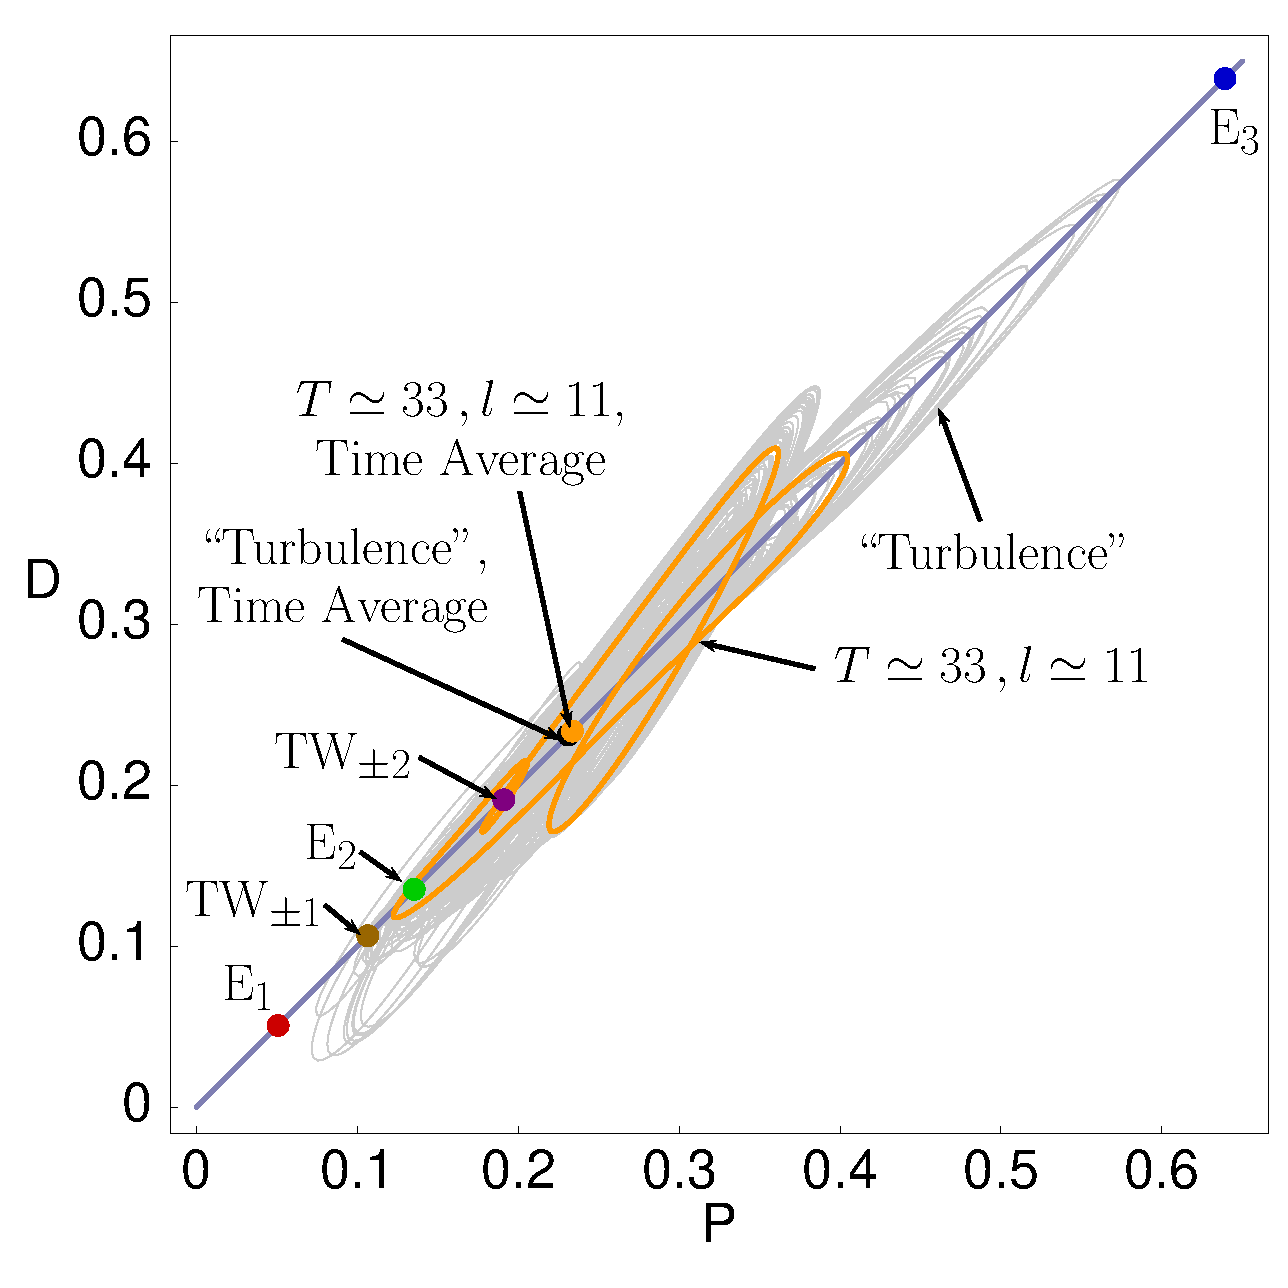
\includegraphics[width=0.46\textwidth, clip=true]{energyBalance_pst}
    & 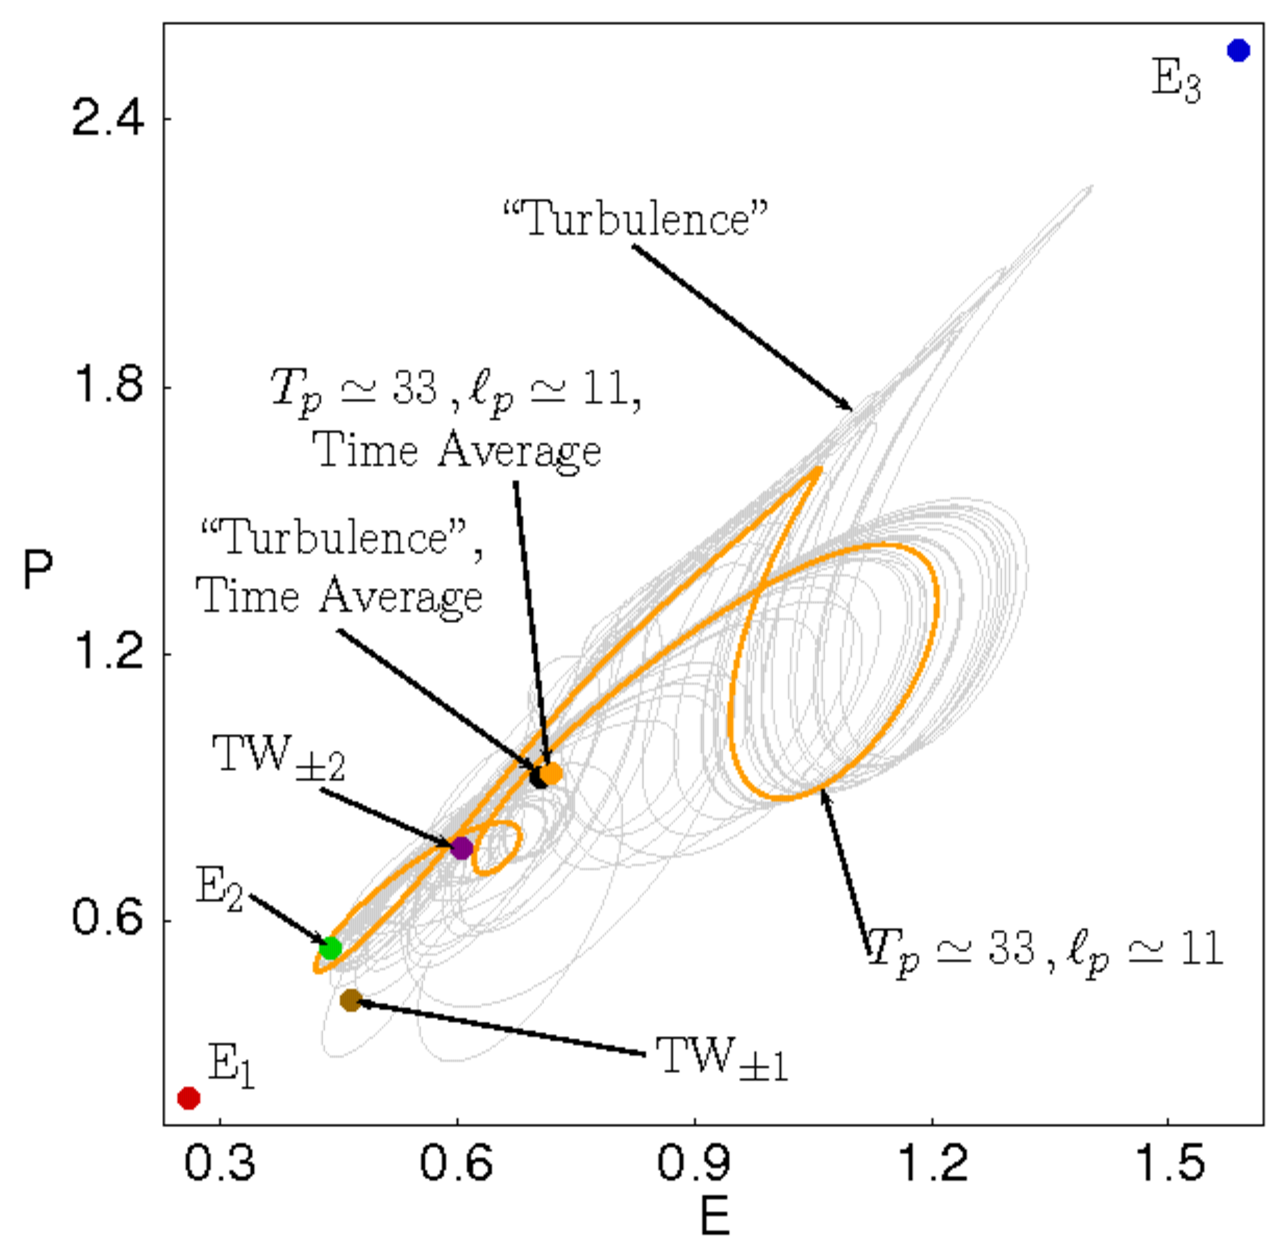
\includegraphics[width=0.46\textwidth, clip=true]{equivaEP_pst}

  \end{tabular}
\end{center}
\caption{
(a) Power input $P$ {\em vs.}
dissipation rate $D$
(b) energy $E$  {\em vs.}
power input $P$,   for several  \eqva\ and \reqva,
a \rpo, and a typical `turbulent' long-time trajectory.
System size $L=22$.
        }
\label{f:drivedrag1}
\end{figure}
%%%%%%%%%%%%%%%%%%%%%%%%%%%%%%%%%%%%%%%%%%%%%%%%%%%%%%%%%%%%%%%%%%

%%%%%%%%%%%%%%%%%%%%%%%%%%%%%%%%%%%%%%%%%%%%%%%%%%%%%%%%%%%%%%%%
\begin{figure}[t]
\begin{center}
 \begin{tabular}{cc}
        ~~~~~~~~(\textit{a})                        &   ~~~~~~~~(\textit{b}) \\
    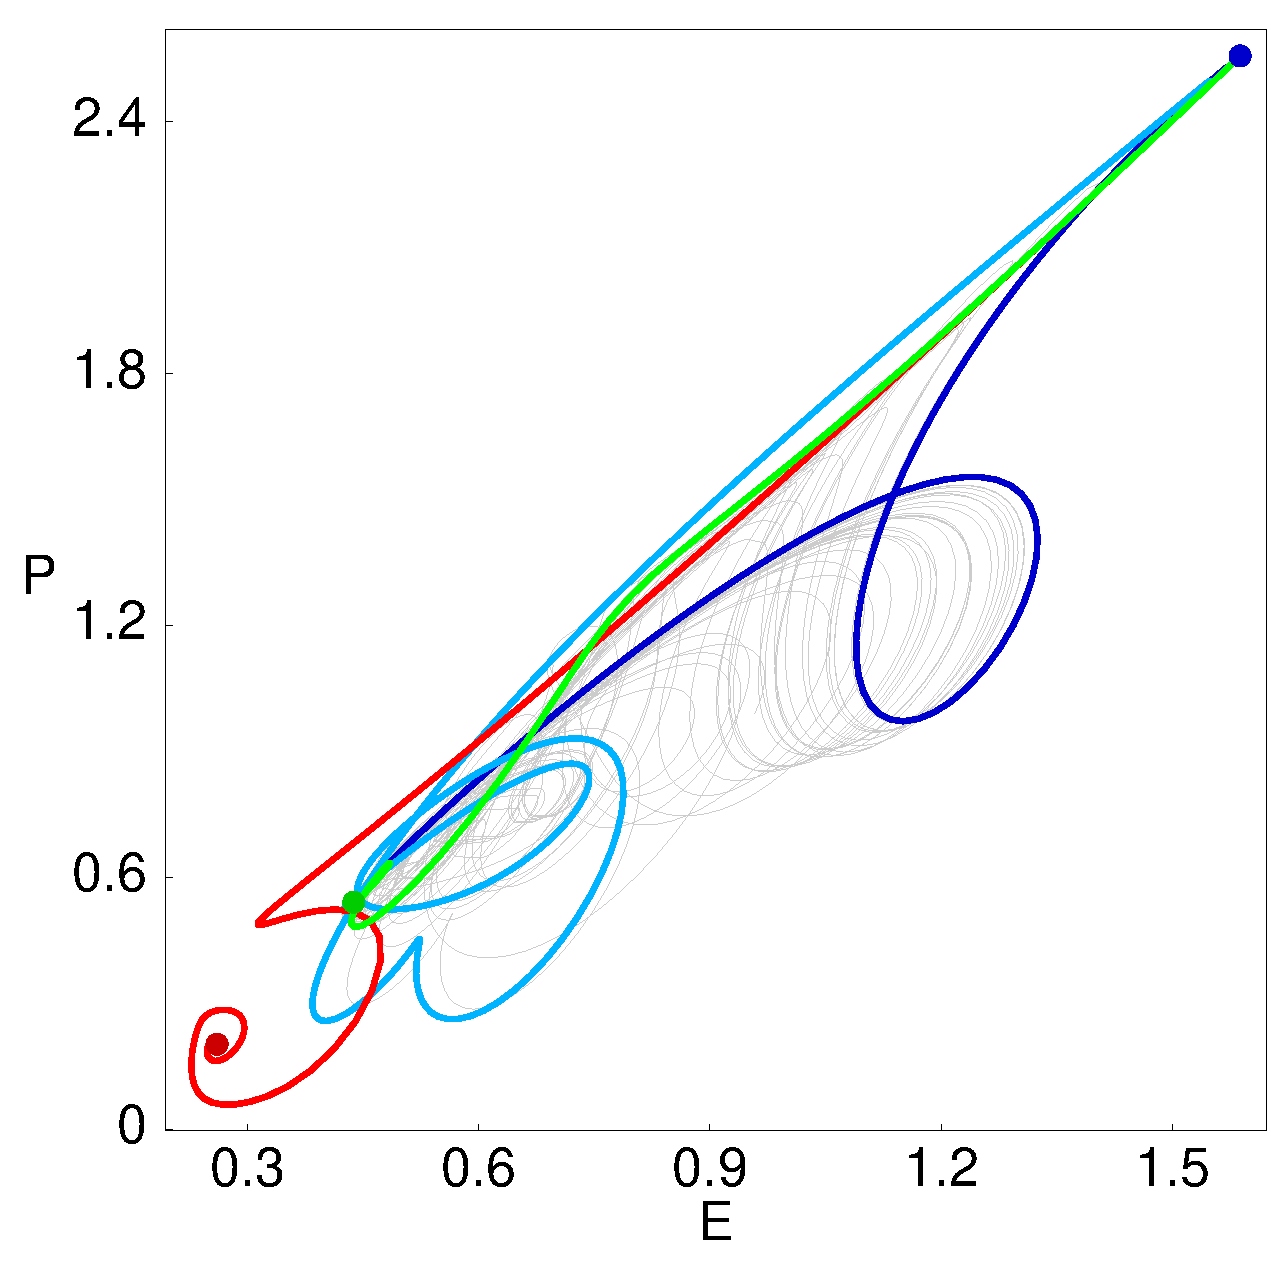
\includegraphics[width=0.46\textwidth, clip=true]{connEP}
     & 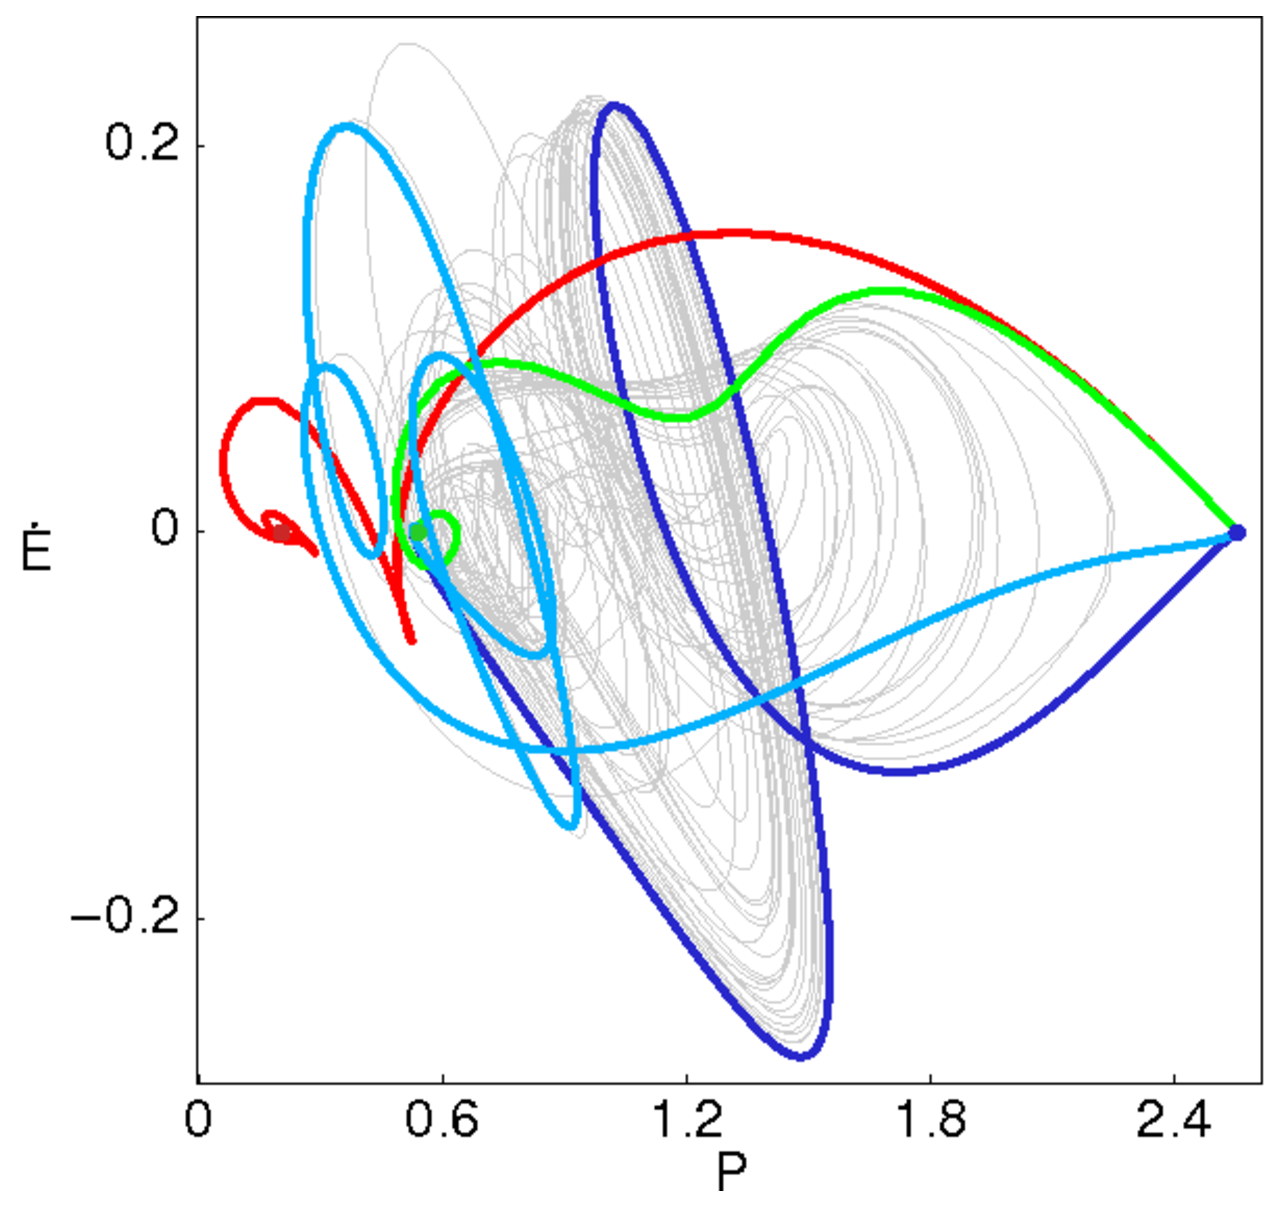
\includegraphics[width=0.46\textwidth, clip=true]{connPEdot}
 \end{tabular}
\end{center}
\caption{
Two projections of the $(E,P,\dot{E})$ representation of the flow.
\EQV{1} (red), \EQV{2} (green), \EQV{3} (blue),
heteroclinic connections from \EQV{2} to $\EQV{3}$ (green),
from $\EQV{1}$ to \EQV{3} (red)
and from \EQV{3} to $\EQV{2}$ (shades of blue), superimposed over
a generic long-time `turbulent' trajectory (grey).
System size $L=22$.
        }
\label{f:drivedragConn}
\end{figure}
%%%%%%%%%%%%%%%%%%%%%%%%%%%%%%%%%%%%%%%%%%%%%%%%%%%%%%%%%%%%%%%%%%

                                                    \toCB
In \reffig{f:drivedrag1} we plot \refeq{EnRate}, the time-dependent
$\dot{\expctE}$ in the power input $P$ {\em vs.}
dissipation rate $D$ plane, for $L=22$ \eqva\ and \reqva,
a selected \rpo, and for a typical `turbulent' long-time
trajectory.

Projections from the $\infty$-dimensional \statesp\ onto the 3-dimensional
$(E,P,D)$ representation of the flow, such as
\reffigs{f:drivedrag1}{f:drivedragConn}, can be misleading.
The most one can say is that if points are clearly separated in an
$(E,P,D)$ plot (for example, in \reffig{f:drivedrag1}
$\EQV{1}$ \eqv\ is outside the recurrent set), they are also separated
in the full \statesp.  Converse is not true -- states of
very different topology can have similar energies.

An example is the \rpo\ $(\period{p},\shift_p) = (32.8,10.96)$
which {is the least unstable short \rpo\ we have detected in this system.
It} appears to be well embedded within the turbulent flow. The mean power
$\timeAver{P_p}$ evaluated as in \refeq{poE}, see \reffig{f:drivedrag1},
is numerically quite close to the long-time turbulent time average
$\timeAver{P}$.

\subsection{Further observables, \KS}
\label{sec:moreObs}

                                                    \toCB
This section contains some material which has not been included in
publications and/or Siminos and Lan Ph.D. theses.

{\bf PC}: believe it or not, we are now set to compute
    $\timeAver{E}$ and $\timeAver{P}$
    using cycle expansions

Substitution % by \refeq{KSeqvCond}
verifies that for an \eqv\ $\expctE$ is constant:
\[
   \dot{\expctE} =
\expct{ \left({u^2}/{2} + u_{x} + u_{xxx} \right) u_x}
    = \expctE \expct{ u_x }=0
    \,.
\]


% PC worked out in part with Bridges
An infinite number of identities for moments of
solutions of KS follow\rf{Bridges_priv}. For example,
integrating by parts $\expct{u_{x} u_t}$,
$\expct{u_{xx} u_t}$,
and
$\expct{u^2 u_t}$,
respectively, one obtains \reqva\ relations
\PC{please re-derive these three. Are there more
    important ones that I have missed?
    Also, I - unnecessarily - specialized to \reqva,
    but these identities will be especially useful for \rpo s}
\RLD{I don't quite follow this process of deriving moments.  What is
the reason we look for some combinations of $u$ and its derivatives?
Why not just take $\expct{u_{x\cdots x}}$?
Is there any physical motivation for such combinations,
beyond $E$, $P$ and $D$?  Maybe use things like $\dot{P}$,
$\dot{D}$, etc.?}
\PC{they merit more thought and time than we have now, so let's
   pick them up after the first paper is submitted}
\bea
% \expct{u_{x} u_t}
%     \qquad \to \qquad
c P &=& \expct{u \, u_{x}{}^2}
\label{Bridges1}\\
c P  &=& \expct{u \, u_{xx}{}^2}
\label{Bridges3}
\,.
\eea
True for any solution:
\bea
% \expct{u_{xx} u_t}
%     \qquad \to \qquad
\dot{P} &=& 2P - \expct{u_{x}{}^3}  - 2 \expct{u_{xxx}{}^2}
\label{PC1}\\
\dot{D} &=& 2\expct{u_{xxxx}{}^2}
    + 5 \expct{u_{xx}{}^2 u_{x}}  - 2 \expct{u_{xxx}{}^2}
\label{PC2} \\
\ddot{E} &=& \dot{P} - \dot{D} =
     2P - \expct{u_{x}{}^3}
    - 2\expct{u_{xxxx}{}^2} - 5 \expct{u_{xx}{}^2 u_{x}}
\label{PC4}\\
\frac{d}{dt} \expct{u_{x}{}^3} &=&
        3 \expct{u_{x}{}^3u + u_{xx}{}^3}
\label{PC5}
\,.
\eea
When moments such as \refeq{Bridges1} are added as
coordinate axes to \reffig{f:drivedragConn}, \reqva\ and
\rpo s are separated from \eqva\ and \po s. Furthermore,
as higher moments have more and more powers of $u$ and derivatives
$u_{xx\cdots x}$, their magnitudes should be strongly suppressed,
providing a symmetry-invariant basis set that can be safely truncated to
a finite-dimensional \statesp.

For example, the energy of \reqva\ \REQV{\pm}{2} which
seems close to the
mean turbulent energy in \reffig{f:drivedrag1} is separated
from it when plotted along the
$\expct{u \, u_{x}{}^2}$ moment, where according to
\refeq{Bridges1} it takes nonzero value $c P$.

%%%%%%%%%%%%%%%%%%%%%%%%%%%%%%%%%%%%%%%%%%%%%%%%%%%%%%%%%%%%%%%%%%%%%%%%%%
% \ifboyscout\else\newpage\fi

\exercise{Channelflow.org.}{ \label{exer:channelflow}
% Predrag                           1apr2013
(Bonus) Please download the code.
\HREF{http://channelflow.org/dokuwiki/doku.php?id=docs:tutorial}{Tutorial}
and
\HREF{http://channelflow.org/dokuwiki/doku.php?id=gtspring2009:howto}
{HowTo}
might be helpful.
        }% end \exercise{\KS\ energy transfer rates
